\section{Diagnostic de l'état de santé des piles à combustible et électrolyseurs}
Il s'agit désormais de s'intéresser à l'état de santé des piles à combustible et des électrolyseurs. Ces composants sont associés pour gérer le stockage de l'énergie électrique sur des périodes de temps plus longues, allant de la semaine à la saison. Cette partie vise à définir un indicateur d'état de santé pour les piles à combustible et les électrolyseurs ainsi que d'apporter une méthode d'estimation de cet état de santé. Cela se fera tout d'abord par une revue de l'état de l'art sur le diagnostic de ces composants, qui permettra de choisir une méthode d'estimation d'état de santé. Cette méthode sera ensuite détaillée dans le cadre du cas d'étude de ce travail, et les résultats qu'elle fournit seront présentés.

\subsection{Choix de l'indicateur d'état de santé}
Plusieurs indicateurs d'état de santé existent pour les piles à combustible et les électrolyseurs, attestant de la dégradation d'au moins une de leurs caractéristiques électriques lorsqu'ils vieillissent. Contrairement aux batteries, ces systèmes ne peuvent pas être associés à des capacités, qui seraient relatives à une possibilité du système à avoir une autonomie. En effet, cet aspect est plutôt dépendant d'une source en hydrogène ou en électricité. Cependant, ces deux systèmes voient tout de même une dégradation de leur caractéristiques en puissance au cours de leur vie \cite{bezmalinovic_characterization_2015}\cite{papakonstantinou_degradation_2020}. Cette dégradation de puissance est plus pertinente à considérer pour le choix de l'indicateur d'état de santé, puisqu'elle est directement déterminante dans la capacité du système hybride à répondre aux besoins en répartition de la puissance du micro-réseau. 

Dans ce travail, l'état de santé (SoH) de la pile à combustible et de l'électrolyseur est représenté par un indicateur scalaire unique reflétant la dégradation de leurs performances par rapport aux conditions nominales de début de vie (\textit{beginng-of-life}, ou BoL). Contrairement aux indicateurs de performance globale de la stratégie de gestion d'énergie (\textit{Energy Management Strategy}, ou EMS), ces définitions visent ici à permettre au système de commande de monitorer l'état des composants en temps réel. L'objectif est d'adapter les lois de contrôle en ajustant les plages de fonctionnement admissibles (puissances minimales et maximales) au fur et à mesure du vieillissement. 

Ainsi, les définitions retenues pour ces deux systèmes s'appuient sur l'évolution de leur caractéristique de puissance à un point de fonctionnement de référence, fixé ici à 75 \% du courant maximal ($i_{max}$) \cite{noauthor_clean_nodate} :

\begin{itemize}
    \item \textbf{Pour la pile à combustible :} le SoH est défini comme le ratio entre la puissance délivrée à l'instant $t$ et la puissance nominale initiale, traduisant ainsi la perte de puissance à courant constant.
    \item \textbf{Pour l'électrolyseur :} le SoH est défini, à l'inverse, comme le rapport entre la puissance électrique consommée au début de vie et celle consommée à l'instant $t$. Cela permet de traduire l'augmentation de la consommation énergétique nécessaire pour produire le même débit d'hydrogène.
\end{itemize}

Ces définitions se traduisent par les expressions suivantes :

\begin{equation}
\text{SoH}_{\text{FC}}(t) = \frac{P_{\text{FC}}(i_{\text{FC,nom,ref}}, t)}{P_{\text{FC}}(i_{\text{FC,nom,ref}}, t=0)}
\label{eq:soh_fc}
\end{equation}

\begin{equation}
\text{SoH}_{\text{ELY}}(t) = \frac{P_{\text{ELY}}(i_{\text{ELY,nom,ref}}, t=0)}{P_{\text{ELY}}(i_{\text{ELY,nom,ref}}, t)}
\label{eq:soh_ely}
\end{equation}

où $i_{\text{FC,nom,ref}}$ et $i_{\text{ELY,nom,ref}}$ correspondent aux courants de référence fixés à 75 \% de la puissance maximale. Un exemple de lecture de ces définitions d'états de santé est visible en figure \ref{soh_pac}

\begin{figure}[h!]
    \centering
    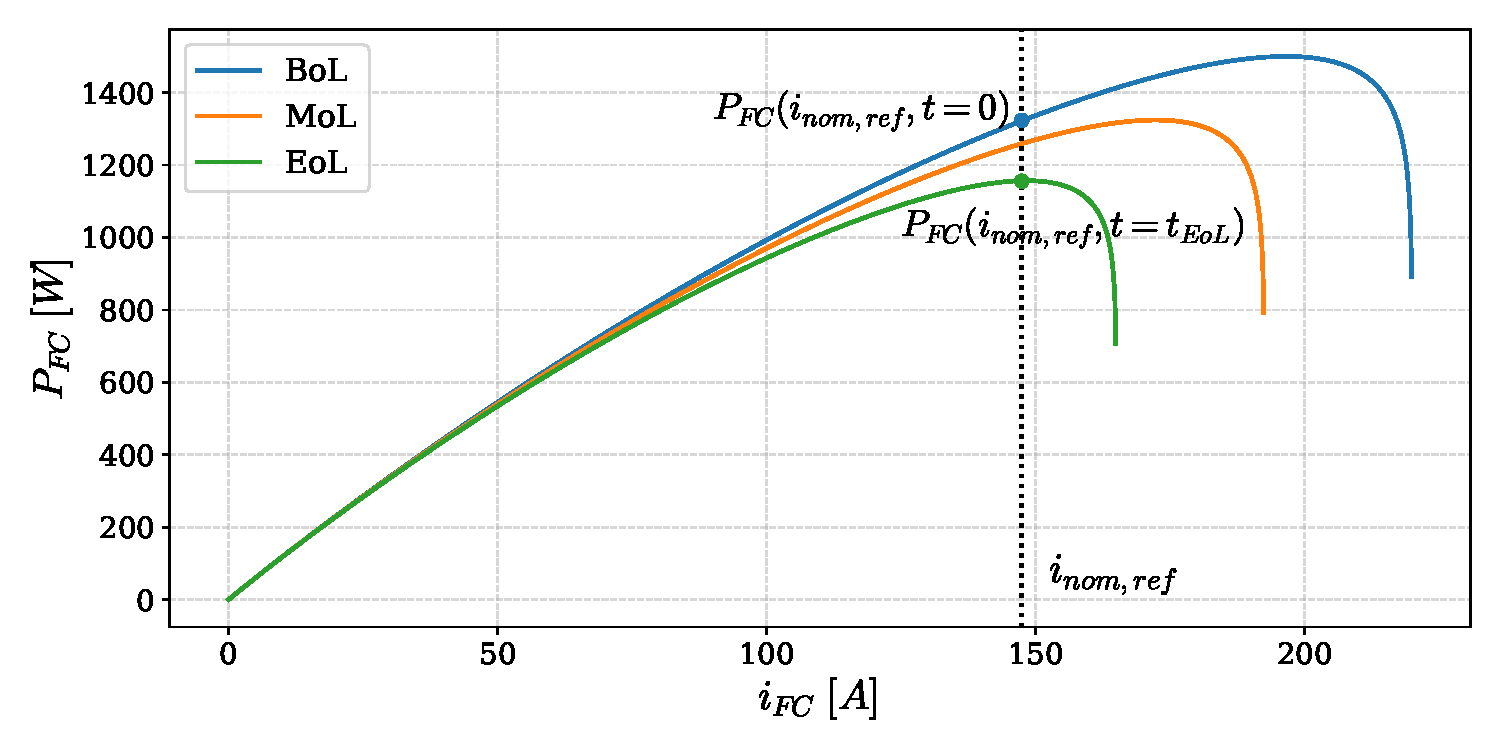
\includegraphics[width=.8\linewidth]{Chapitre 1/Diag_pac/Figures/P_fc_vs_i_fc.pdf}
    \caption{Évolution des courbes de polarisation d'une PEMFC (début, milieu et fin de vie), et de la puissance considérée pour le courant nominal de référence}
    \label{soh_pac}
\end{figure}
\FloatBarrier
Une fois ces métriques établies, il convient d'identifier les méthodes permettant leur évaluation au cours du temps.

\subsection{État de l'art des méthodes d'estimation en ligne}

Avec les définitions retenues, le courant de référence $i_{\text{ref}}$ étant constant, la puissance est directement proportionnelle à la tension ($P = U \cdot i_{\text{ref}}$). Le SoH peut donc être exprimé comme un ratio de tension. Cette formulation est cohérente avec les critères de fin de vie usuels, souvent exprimés tension. Cela est également le cas pour le PEMWE où une dérive de tension de $10\,\%$ correspond ici à un SoH d'environ $90,9\,\%$ \cite{dittmar_prognostics_2025}.

Le principal verrou de l'estimation en ligne réside dans le fait que le système n'opère que rarement à $i_{\text{ref}}$. L'objectif des méthodes présentées est donc de reconstruire la tension au point de référence à partir de mesures en régime dynamique, soit via une courbe de polarisation, soit via des paramètres équivalents. Trois grandes familles se distinguent : les approches paramétriques, la SIE et les approches orientées données.

% ---------------------------------------------------------

\subsubsection{Identification paramétrique en ligne et filtrage récursif}

Les modèles semi-empiriques permettent d'exprimer la tension comme fonction paramétrée du courant, dont les coefficients évoluent avec le vieillissement \cite{hao_improved_2016, sun_pemfc_2025}.

L'estimation en ligne consiste alors à identifier ces paramètres à partir des mesures disponibles. Les méthodes de régression récursive (\textit{Recursive Least Squares}, ou RLS) offrent une solution simple pour des modèles linéarisés, mais restent limitées face aux non-linéarités. Les filtres bayésiens (EKF, \textit{Unscented Kalman Filter} UKF...) permettent de traiter explicitement ces non-linéarités en formulant le problème comme une estimation d'état, où les paramètres sont considérés comme des variables dynamiques \cite{bressel_extended_2016, pene_aging_2025}. Le filtre particulaire constitue une extension plus générale, au prix d'un coût de calcul élevé \cite{guo_marginalized_2023}.

Ces paramètres équivalents estimés, il devient alors possible de reconstruire la tension du système et extrapoler $U(i_{\text{ref}}, t)$, fournissant ainsi une estimation directe du SoH. Des formulations récentes basées sur des régressions séparables permettent d'améliorer la robustesse et la convergence en conditions dynamiques \cite{beltran_online_2024}. Pour le PEMWE, des approches de régression transférée ont également été proposées pour stabiliser l'estimation \cite{yan_state--health_2024}.

% ---------------------------------------------------------

\subsubsection{Méthodes basées sur la spectroscopie d'impédance électrochimique (SIE)}

La SIE permet de décorréler les contributions des différentes surtensions par analyse fréquentielle \cite{ma_review_2025}. Le spectre d'impédance est généralement interprété via un circuit électrique équivalent, dont les paramètres constituent des indicateurs physiques de dégradation (résistance ohmique, transfert de charge, diffusion).

Certains de ces paramètres peuvent être reliés indirectement à la tension : la résistance de haute fréquence permet par exemple d'estimer la contribution ohmique, tandis que la résistance de transfert de charge reflète les pertes d'activation. Des travaux récents ont montré la possibilité d'estimer ces paramètres en ligne, notamment en utilisant des excitations multi-sine ou les ondulations des convertisseurs de puissance \cite{xie_impedance_2023}. Couplée à des méthodes d'identification récursive, la SIE permet ainsi de suivre l'évolution des paramètres équivalents \cite{kim_application_2025}.

De la même manière que les méthodes de régression ou de filtrage, les paramètres équivalents obtenus permettent ainsi de reconstruire le profil de tension du système. La SIE reste cependant plus difficile à mettre en oeuvre, étant naturellement plus intrusive et sensible au bruit, ce qui limite son utilisation en continu. Elle est donc le plus souvent utilisée comme outil de diagnostic ponctuel ou de recalibration.

% ---------------------------------------------------------

\subsubsection{Méthodes orientées données}

Les approches orientées données visent à apprendre directement la relation entre les variables mesurées et la tension, sans modèle physique explicite. Des méthodes telles que les réseaux de neurones (\textit{Long Short-Term Memory}, ou LSTM) ou les modèles à noyaux (\textit{Gaussian Process}, ou GPR, SVM) permettent de reconstruire la tension en conditions dynamiques \cite{li_health_2024}\cite{zhang_deep_2024}\cite{nagulapati_machine_2023}.

Ces méthodes offrent une bonne capacité de modélisation des non-linéarités, mais présentent des limites importantes pour l'estimation du SoH, notamment sur le manque d'interprétabilité, la dépendance aux données d'entraînement et la difficulté d'extrapolation hors domaine. 

% ---------------------------------------------------------

\subsubsection{Bilan et positionnement de l'approche retenue}

Les méthodes paramétriques associées à un filtrage récursif constituent aujourd'hui l'approche la plus adaptée à une estimation continue du SoH, car elles permettent une reconstruction directe de la tension au point de référence à partir de mesures limitées. La SIE offre une information physiquement riche mais reste difficile à exploiter en continu, tandis que les approches orientées données présentent un fort potentiel mais souffrent encore de limitations en robustesse et en généralisabilité.

Le tableau~\ref{tab:soh_methods} synthétise ces approches. Pour le PEMWE, bien que moins mature, les travaux récents convergent vers des indicateurs similaires, notamment la tension à courant fixé et la résistance ohmique \cite{dittmar_prognostics_2025}\cite{makhsoos_proton_2025}.

\begin{table}[h]
\centering
\caption{Synthèse des méthodes d'estimation en ligne du SoH issues de la littérature\vspace{0.15cm} }
\begin{tabular}{M{3cm} M{4.2cm} M{3cm} M{3.6cm} }
\hline
\textbf{Méthodes} & \textbf{Exemples \& Références} & \textbf{Avantages} & \textbf{Inconvénients} \\
\hline \hline
\multirow{6}{3cm}{\centering Identification paramétrique et filtrage récursif} 
& Identification RLS \& modèles semi-empiriques \cite{hao_improved_2016, sun_pemfc_2025} & \multirow{6}{2.5cm}{\centering Reconstruction directe de $U(i_{\text{ref}})$, adaptée au suivi continu} & \multirow{6}{2.5cm}{\centering Dépendant de la validité du modèle physique, coût calcul (PF)} \\
\cline{2-2}
& Filtrage bayésien (EKF, UKF) \cite{bressel_extended_2016}\cite{pene_aging_2025} &  &  \\
\cline{2-2}
& Filtre particulaire (PF) \cite{guo_marginalized_2023} &  &  \\
\cline{2-2}
& Régressions robustes et transférées \cite{beltran_online_2024}\cite{yan_state--health_2024} &  &  \\
\hline
\multirow{4}{3cm}{\centering Spectroscopie d'impédance électrochimique} 
& \vspace{0.15cm} Analyse par circuit électrique équivalent \cite{ma_review_2025} \vspace{0.15cm} & \multirow{4}{2.5cm}{\centering Information physique riche, décorrélation des surtensions} & \multirow{4}{3cm}{\centering Intrusive, sensible au bruit, difficile à mettre en œuvre en continu} \\
\cline{2-2}
& \vspace{0.15cm} Estimation via ondulations de courant ou multi-sine \cite{xie_impedance_2023}\cite{kim_application_2025} \vspace{0.15cm} &  &  \\
\hline
\multirow{3}{3cm}{\centering Approches orientées données} 
& \vspace{0.2cm} Réseaux de neurones (LSTM) \cite{li_health_2024}\cite{zhang_deep_2024}\vspace{0.2cm} & \multirow{3}{2.5cm}{\centering Bonne gestion des non-linéarités, pas de modèle explicite}\vspace{0.18cm}  & \multirow{3}{3cm}{\centering Manque d'interprétabilité, dépendance aux données, faible extrapolation}\vspace{0.18cm}  \\
\cline{2-2}
& \vspace{0.2cm} Modèles à noyaux (GPR, SVM) \cite{nagulapati_machine_2023} \vspace{0.2cm} &  &  \\
\hline
\end{tabular}
\label{tab:soh_methods}
\end{table}
\FloatBarrier

Au regard de ce panorama, l'approche retenue dans ce manuscrit repose sur l'identification paramétrique en ligne via un EKF couplé à un modèle physique. Cette méthode permet de reconstruire explicitement la courbe de polarisation et d'en extraire la puissance au point de référence à tout instant, offrant un bon compromis entre précision, interprétabilité physique et coût de calcul pour une implémentation en ligne.


% ============================================================
%  CHAPITRE 2 — Sous-sections sur le modèle de vieillissement
%  et l'estimation par filtre de Kalman étendu
%  À intégrer dans le chapitre, après la description du modèle
%  macroscopique du système.
%
%  Structure :
%    \subsection{Modèle de vieillissement des composants}
%    \subsection{Estimation par filtre de Kalman Étendu}
%      \subsubsection{Principe}
%      \subsubsection{Application à la pile à combustible et à l'électrolyseur}
%    \subsection{Discussion}
%    \subsection{Limitations}
% ============================================================

% ------------------------------------------------------------
\subsection{Modèle de vieillissement des composants}
% ------------------------------------------------------------
Afin d'appliquer l'estimation d'état de santé par filtre de Kalman étendu, il est tout d'abord nécessaire de poser un modèle physique, dépendant du vieillissement, des composants. L'approche retenue ici est dans la lignée des modèles établis dans la littérature pour des applications similaires ~\cite{bressel_extended_2016}\cite{abdin_modelling_2015}.

\paragraph{Modèle de vieillissement de la PEMFC.}

Le modèle de tension d'un stack d'une pile à combustible retenu est fondé sur des travaux passés bien établis~\cite{bressel_extended_2016}, dont l'expression est rappelée à l'équation~\ref{eq:pemfc_voltage_nominal}. Ce modèle repose sur la courbe de polarisation, qui traduit la tension en sortie du stack en fonction du courant et de la température~:

\begin{equation}
    V_{\text{st}} = n_s \left( E_0 - Ri - AT\ln\left(\frac{\frac{i}{S} + j_{\text{in}}}{j_0}\right) - BT\ln\left(1 - \frac{i}{Sj_L}\right) \right)
    \label{eq:pemfc_voltage_nominal}
\end{equation}

où $n_s$ est le nombre de cellules en série, $E_0$ la tension à vide d'une cellule [V], $R$ la résistance interne [$\Omega$], $j_0$ et $j_L$ respectivement la densité de courant d'activation et la densité de courant limite [A/m$^2$], $A$ la constante des pertes par activation [V/K], $j_{\text{in}}$ la densité de courant résiduelle [A/m$^2$], $B$ la constante des pertes par concentration [V/K], $S$ la surface active [m$^2$] et $T$ la température [K]. Le courant $i$ est ici toujours positif. Ce modèle produit la courbe de polarisation caractéristique d'une PEMFC, illustrée à la Figure~\ref{fig:pemfc_polar}, faisant apparaître les trois régimes de pertes classiques~: pertes d'activation aux faibles courants, pertes ohmiques en régime intermédiaire, et pertes de concentration aux forts courants.

\begin{figure}[h!]
    \centering
    % placeholder — courbe de polarisation PEMFC
    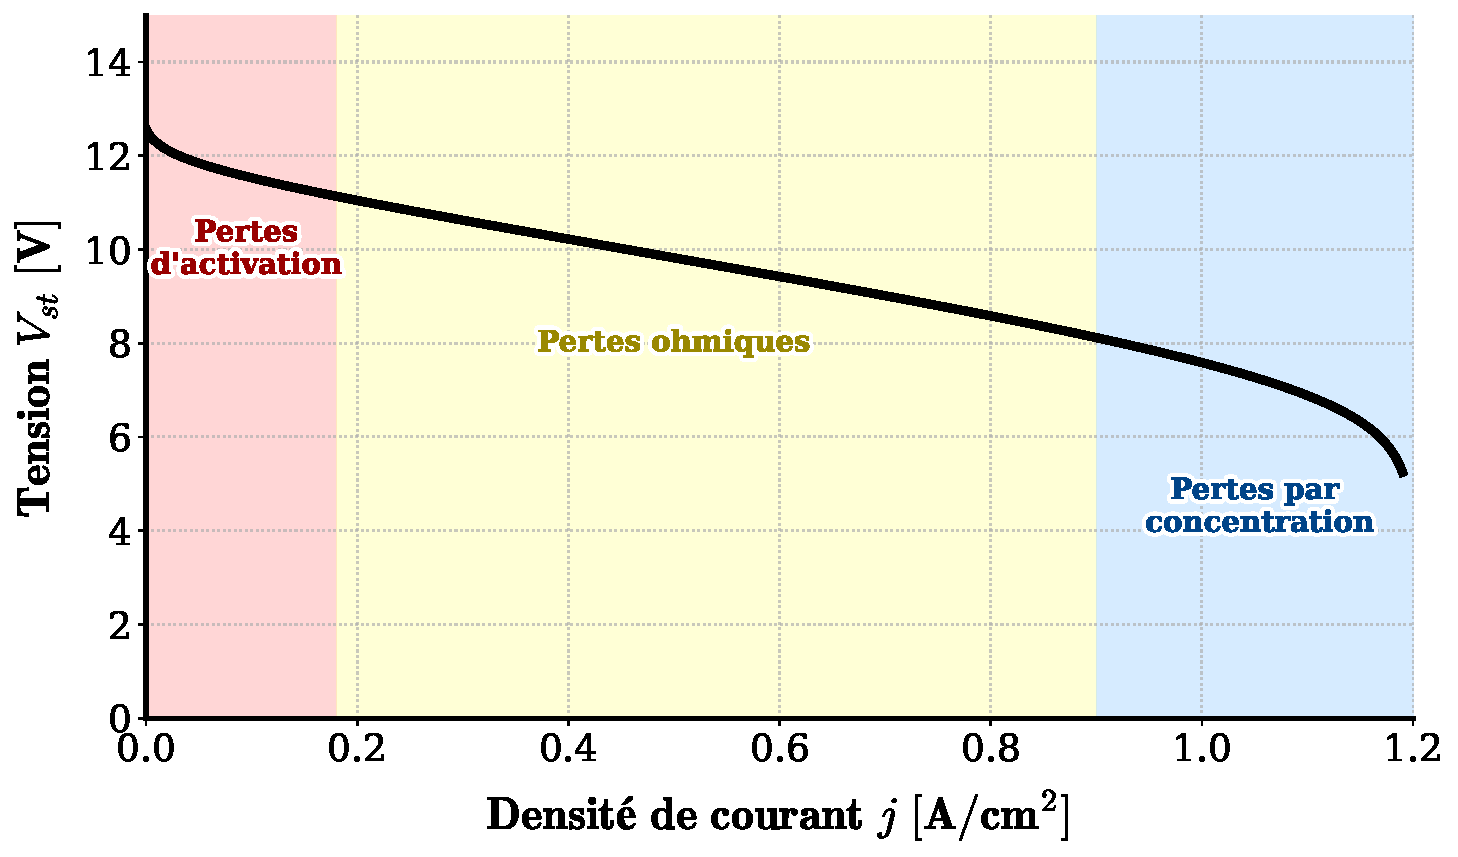
\includegraphics[width=0.8\linewidth]{Chapitre 1/Diag_pac/Figures/PEMFC_Polarization_Curve.pdf}
    \caption{Courbe de polarisation d'un stack de pile à combustible~: mise en évidence des trois régimes de pertes.}
    \label{fig:pemfc_polar}
\end{figure}
\FloatBarrier

Il est empiriquement vérifié dans la littérature que, parmi les quatre paramètres de ce modèle, deux varient grandement avec le temps d'utilisation~: la résistance interne $R$ et le courant limite $j_L$~\cite{bressel_extended_2016}\cite{foniok_mechanisms_2025}. Ces évolutions peuvent être considérées comme linéaires et sont généralement couplées sous un unique paramètre scalaire $\alpha_{\text{FC}}$ [-], représentant le niveau de dégradation de la pile~:

\begin{equation}
    R = R_0 (1 + \alpha_{\text{FC}}) \qquad \| \qquad j_L = j_{L,0}(1 - \alpha_{\text{FC}})
    \label{eq:pemfc_aging_params}
\end{equation}

Le paramètre $\alpha_{\text{FC}}$ est nul en début de vie et croît au fil de l'utilisation~: une augmentation de $\alpha_{\text{FC}}$ se traduit simultanément par une hausse de la résistance interne (pertes ohmiques accrues) et une réduction du courant limite (apparition précoce des pertes de concentration). Ces deux effets contribuent à une chute de la tension de sortie à courant donné, c'est-à-dire à une dégradation des performances. Le modèle de tension modifié intégrant le vieillissement devient ainsi~:

\begin{equation}
    V_{\text{st}} = n_s \left( E_0 - R_0(1+\alpha_{\text{FC}})i - AT\ln\left( \frac{\frac{i}{S} + j_{\text{in}}}{j_0}\right) - BT\ln\left(1 - \frac{i}{Sj_{L,0}(1-\alpha_{\text{FC}})}\right) \right)
    \label{eq:pemfc_voltage_aging}
\end{equation}

L'état de santé de la PEMFC est alors directement relié à $\alpha_{\text{FC}}$, étant donné qu'une détermination de ce paramètre permet une reconstruction de la courbe de polarisation et donc une détermination de la puissance pour un courant de référence.

\paragraph{Modèle de vieillissement du PEMWE.}

Par analogie avec la PEMFC, le modèle de tension de l'électrolyseur PEM repose sur une courbe de polarisation de structure similaire, mais dont la physique est inversée~: l'électrolyseur consomme de l'électricité pour produire de l'hydrogène, si bien que sa tension de fonctionnement est supérieure à la tension réversible. Le modèle nominal de tension du PEMWE s'écrit~\cite{abdin_modelling_2015}~:

\begin{equation}
    V_{\text{st}} = n_s \left( E_0 + R|i| + AT\left(\ln\frac{\frac{|i|}{S} + j_{\text{in}}}{j_0}\right) + BT\ln\left(1 - \frac{|i|}{S \cdot j_L}\right) \right)
    \label{eq:pemwe_voltage_nominal}
\end{equation}

où les paramètres ont la même signification que dans le modèle PEMFC. Le courant $i$ est ici toujours négatif par convention. La courbe de polarisation caractéristique de l'électrolyseur, illustrée à la Figure~\ref{fig:pemwe_polar}, fait apparaître les surtensions d'activation, ohmiques et de concentration, qui s'additionnent à la tension réversible.

\begin{figure}[h!]
    \centering
    % placeholder — courbe de polarisation PEMWE
    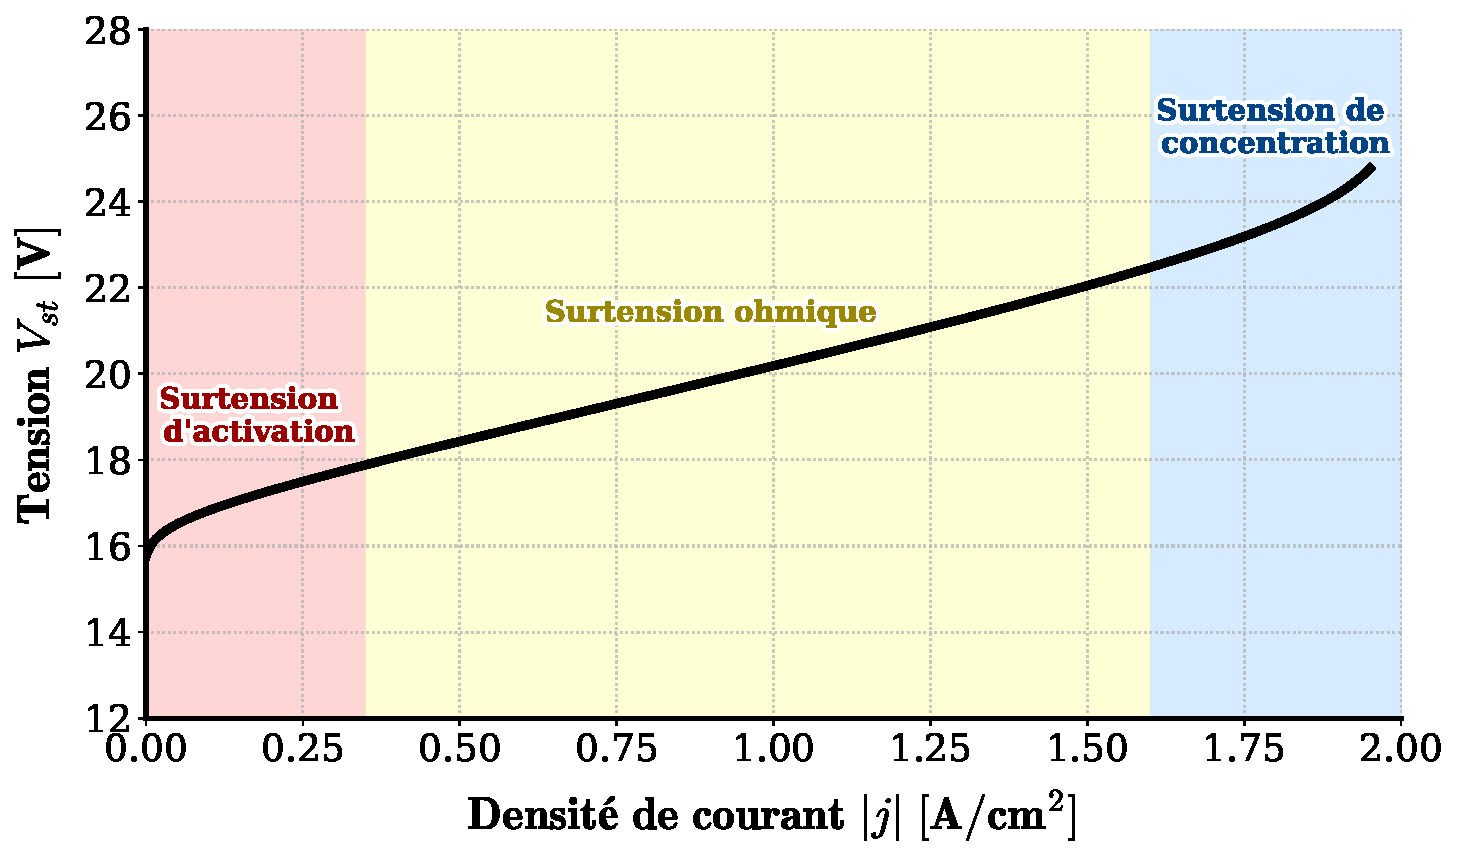
\includegraphics[width=0.8\linewidth]{Chapitre 1/Diag_pac/Figures/PEMWE_Polarization_Curve.pdf}
    \caption{Courbe de polarisation d'un stack d'électrolyseur~: mise en évidence des trois surtensions caractéristiques.}
    \label{fig:pemwe_polar}
\end{figure}
\FloatBarrier

Par analogie avec la démarche adoptée pour la PEMFC, le vieillissement de l'électrolyseur est modélisé par un paramètre scalaire $\alpha_{\text{ELY}}$, qui agit sur la résistance interne et sur le courant limite selon~:

\begin{equation}
    R = R_0 (1 + \alpha_{\text{ELY}}) \qquad \| \qquad j_L = j_{L,0}(1 - \alpha_{\text{ELY}})
    \label{eq:pemwe_aging_params}
\end{equation}

Une augmentation de $\alpha_{\text{ELY}}$ se traduit par une hausse de la tension de fonctionnement à courant donné, c'est-à-dire par une consommation électrique accrue pour produire la même quantité d'hydrogène~: le composant devient moins efficace énergétiquement. Le modèle de tension du PEMWE intégrant le vieillissement s'écrit alors~:

\begin{equation}
    V_{\text{st}} = n_s \left( E_0 + R_0(1+\alpha_{\text{ELY}})|i| + AT\ln\left(\frac{\frac{|i|}{S} + j_{\text{in}}}{j_0}\right) + BT\ln\left(1 - \frac{|i|}{S \cdot j_{L,0}(1-\alpha_{\text{ELY}})}\right) \right)
    \label{eq:pemwe_voltage_aging}
\end{equation}
De manière symétrique à la PEMFC, l'information sur l'état de santé est ici intrinsèquement liée à $\alpha_{\text{ELY}}$, et c'est sa détermination qui permet de reconstruire la courbe de polarisation et donc d'en déduire la puissance électrique nécessaire pour le courant de référence.

Cette formulation unifiée pour les deux composants hydrogène présente l'avantage de la cohérence~: un même formalisme de vieillissement est appliqué à la PAC et à l'électrolyseur, seul le signe des effets physiques changeant. Dans les deux cas, $\alpha = 0$ correspond à un composant neuf et un $\alpha$ croissant représente le vieillissement des composants. Il est à noter ici que les deux modèles présentés fonctionnent à température constante.

% ------------------------------------------------------------
\subsection{Estimation par filtre de Kalman Étendu}
% ------------------------------------------------------------

% - - - - - - - - - - - - - - - - - - - - - - - - - - - - - -
\subsubsection{Principe}
% - - - - - - - - - - - - - - - - - - - - - - - - - - - - - -

Le paramètre de vieillissement $\alpha$ n'est pas directement accessible par une mesure physique simple. En pratique, on ne dispose que de mesures de tension, de courant et, éventuellement, de température. Il s'agit donc d'estimer ce paramètre à partir de ces observables, ce qui constitue un problème d'estimation d'état non linéaire. L'algorithme du filtre de Kalman étendu a été retenu dans ce but~: il a en effet déjà fait ses preuves notamment pour les systèmes de piles à combustible~\cite{bressel_extended_2016}\cite{chen_fuel_2019}, et sa structure en temps discret est directement compatible avec une implémentation numérique.

L'état du système estimé est composé de deux paramètres~: $\alpha_k$, le paramètre de vieillissement à l'instant discret $k$, et $\beta_k$, sa vitesse de dégradation. Ces deux paramètres forment le vecteur d'état $\mathbf{x}_k = [\alpha_k \; \beta_k]^T$. N'ayant pas de modèle explicite de l'évolution de $\beta$, celle-ci est supposée quasi constante sur une période d'échantillonnage~: $\beta_k \approx \beta_{k-1}$. Le système d'équations en temps discret s'écrit alors~:

\begin{equation}
    \mathbf{x}_k = A\mathbf{x}_{k-1} + \mathbf{w}_{k-1}
    \label{eq:ekf_state}
\end{equation}
\begin{equation}
    y_k = g(\mathbf{x}_k, u_k) + v_k
    \label{eq:ekf_output}
\end{equation}

où $y_k$ représente la tension du stack mesurée à l'instant $k$, $g$ est la fonction non linéaire représentant le modèle de tension avec vieillissement (eq.~\ref{eq:pemfc_voltage_aging} ou~\ref{eq:pemwe_voltage_aging}), $u_k$ représente les entrées de commande (courant et température), et $\mathbf{w}_k$, $v_k$ sont des bruits gaussiens à moyenne nulle. La matrice de transition $A$ à temps discret s'écrit~:

\begin{equation}
    A = \begin{bmatrix} 1 & T_s \\ 0 & 1 \end{bmatrix}
    \label{eq:ekf_transition}
\end{equation}

où $T_s$ est la période d'échantillonnage de l'algorithme. L'algorithme de l'EKF se déroule en trois étapes successives à chaque instant $k$, résumées dans le Tableau~\ref{tab:ekf}~:

\begin{table}[h!]
\centering
\caption{Algorithme du filtre de Kalman étendu.}
\label{tab:ekf}
\begin{tabularx}{\textwidth}{lXX}
\hline
\textbf{(i) Initialisation} & \textbf{(ii) Prédiction} & \textbf{(iii) Correction} \\
\hline
$\mathbf{x}_{0|0} = \mathbf{0}$ &
$\mathbf{x}_{k|k-1} = A\mathbf{x}_{k-1|k-1}$ &
$\mathbf{x}_{k|k} = \mathbf{x}_{k|k-1} + K_k\bigl(V_{\text{st},k} - g(\mathbf{x}_{k|k-1}, u_k)\bigr)$ \\
$P_{0|0} = 0$ &
$P_{k|k-1} = AP_{k-1|k-1}A^T + Q$ &
$P_{k|k} = (I - K_k H_k)P_{k|k-1}$ \\
& &
où~: $K_k = P_{k|k-1}H_k^T\bigl(H_k P_{k|k-1}H_k^T + R_v\bigr)^{-1}$ \\
& & et~: $H_k = \dfrac{\partial g(\mathbf{x}_k, u_k)}{\partial \mathbf{x}_k}$ \\
\hline
\end{tabularx}
\end{table}

où $Q$ est la matrice de covariance du bruit de procédé associée à $\mathbf{w}_k$, $R_v$ est la matrice de covariance du bruit de mesure associée à $v_k$, $P_{k|k}$ est la matrice de covariance de l'erreur d'estimation, et $H_k$ est la matrice jacobienne de $g$ par rapport à l'état $\mathbf{x}_k$. À chaque pas, la phase de prédiction propage l'état estimé selon la dynamique du modèle, et la phase de correction le recale grâce à la mesure de tension disponible, via le gain de Kalman $K_k$. Ici le premier coefficient diagonal de la matrice $P_{k|k}$ représente l'écart-type de l'erreur sur l'observation et permet ainsi de reconstruire les intervalles de confiance autour du paramètre de vieillissement $\alpha_k$.

% - - - - - - - - - - - - - - - - - - - - - - - - - - - - - -
\subsubsection{Application à la pile à combustible et à l'électrolyseur}
% - - - - - - - - - - - - - - - - - - - - - - - - - - - - - -

L'algorithme décrit ci-dessus est appliqué séparément à chacun des deux composants hydrogène, en utilisant le modèle de tension avec vieillissement correspondant comme fonction d'observation $g$. Il est considéré que le reste des paramètres du modèle (nombre de cellules $n_s$, tension à vide $E_0$, résistance interne $R_0$, densité de courant d'activation $j_0$, densité de courant limite $j_L$, constantes des pertes par activation $A$ et par concentration $B$, surface active $S$) sont connus, que ce soit par le fournisseur du composant ou par reconstruction par une courbe de polarisation en début de vie. Pour rappel, la température est ici constante. Les paramètres $\alpha$ sont donc les seuls inconnues des modèles. Un modèle du micro-réseau basé sur la représentation énergétique macroscopique (REM) a été développé sous Matlab/Simulink\textsuperscript{\textregistered}\ afin de simuler l'évolution en temps réel du micro-réseau (fig. \ref{fig:emr_mg}). La REM est un formalisme graphique de modélisation basé qui met l'accent sur les échanges énergétiques entre des systèmes connectés \cite{lenoir_electric_2023}.
\begin{figure}[h!]
    \centering
    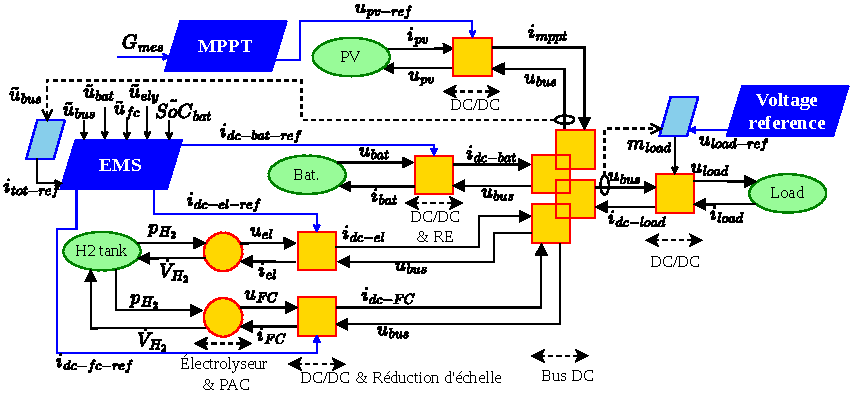
\includegraphics[width=\linewidth]{Chapitre 1/Diag_pac/Figures/EMR_MG_v8.pdf}
    \caption{Représentation énergétique macroscopique du micro-réseau}
    \label{fig:emr_mg}
\end{figure}
\FloatBarrier
Dans ce modèle sont ensuite introduits deux vieillissement pour le moment exogènes, par le biais des paramètres $\alpha$, qui auront pour effet de modifier les caractéristiques statiques des PEMFC et PEMWE. L'application de l'EKF dans ce système permet ainsi une comparaison entre l'évolution de la valeur réelle de $\alpha$ et sa valeur estimée par l'observateur.


\paragraph{Application à la PEMFC.}
Pour la pile à combustible, la fonction $g$ est donnée par l'équation~\ref{eq:pemfc_voltage_aging}. Le jacobien $H_k$ est calculé analytiquement en dérivant cette expression par rapport aux composantes du vecteur d'état $[\alpha_k, \beta_k]^T$. Seule la dérivée par rapport à $\alpha_k$ est non nulle, $\beta_k$ n'apparaissant pas explicitement dans $g$~:

\begin{equation}
    \frac{\partial g_{\text{FC}}}{\partial \alpha_k} = n_s \left( -R_0 i - \frac{BTi}{Sj_{L,0}(1-\alpha_k) - i/S} \right)
    \label{eq:ekf_jacobian_fc}
\end{equation}

Les résultats de simulation illustrés à la Figure~\ref{fig:ekf_fc} montrent que l'état de santé estimé par l'algorithme est fidèle au paramètre de vieillissement réel introduit dans la simulation. On observe que lors des phases où le courant de la pile à combustible est nul, l'influence de $\alpha$ devient nulle dans le modèle (eq.~\ref{eq:pemfc_voltage_aging}), ce qui prive temporairement l'algorithme d'information~: un léger décalage peut alors s'installer, qui se résorbe rapidement dès que le composant est à nouveau sollicité~\cite{lenoir_diagnostic_2024}.

\begin{figure}[h!]
    \centering
    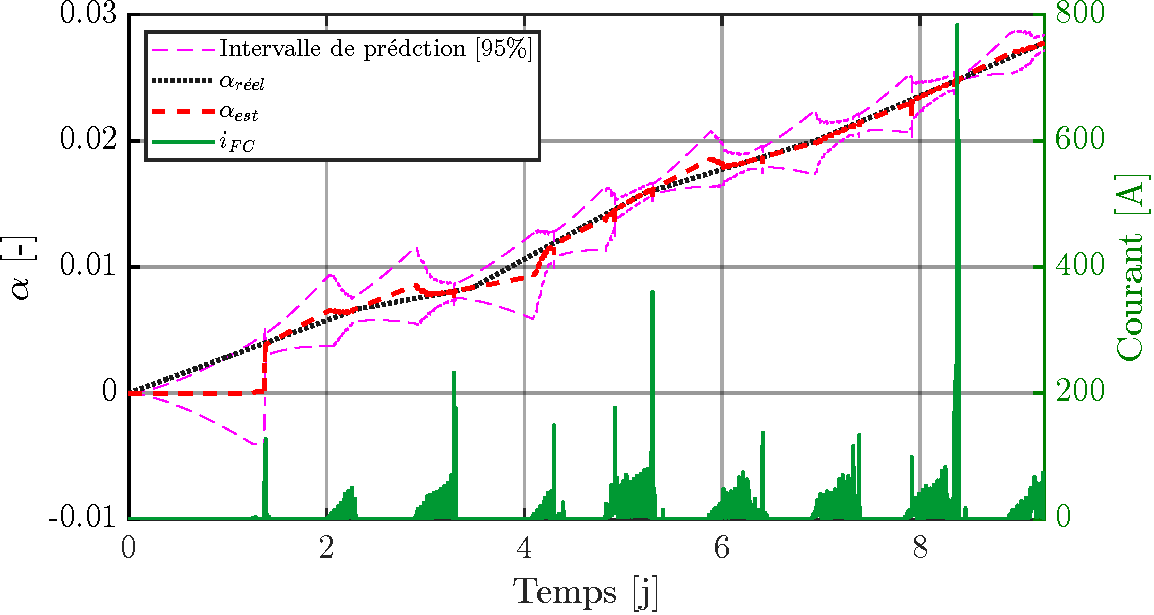
\includegraphics[width=\linewidth]{Chapitre 1/Diag_pac/Figures/comp_alpha_sigma_pemfc.pdf}
    \caption{Comparaison entre le paramètre de vieillissement réel $\alpha$ et son estimation par l'EKF pour la PEMFC, mise en regard avec le courant de la pile à combustible.}
    \label{fig:ekf_fc}
\end{figure}
\FloatBarrier

\paragraph{Application au PEMWE.}
Pour l'électrolyseur, la même structure d'EKF est utilisée, la fonction $g$ étant cette fois donnée par l'équation~\ref{eq:pemwe_voltage_aging}. Le jacobien est calculé de manière analogue~:

\begin{equation}
    \frac{\partial g_{\text{ELY}}}{\partial \alpha_k} = n_s \left( R_0 |i| - \frac{BT|i|}{S \cdot j_{L,0}(1-\alpha_k) - |i|/S} \right)
    \label{eq:ekf_jacobian_ely}
\end{equation}

L'extension du formalisme à l'électrolyseur est rendue possible par la symétrie des modèles de tension~: la PEMFC et le PEMWE partagent la même structure paramétrique, avec simplement un signe inversé sur les termes de surtension. Il est ainsi justifié de considérer que la méthode d'estimation développée pour la pile à combustible se transpose directement à l'électrolyseur par inversion du modèle~\cite{abdin_modelling_2015}. Un résultat de simulation analogue à celui présenté pour la PEMFC est illustré à la figure \ref{fig:ekf_ely}.

\begin{figure}[h!]
    \centering
    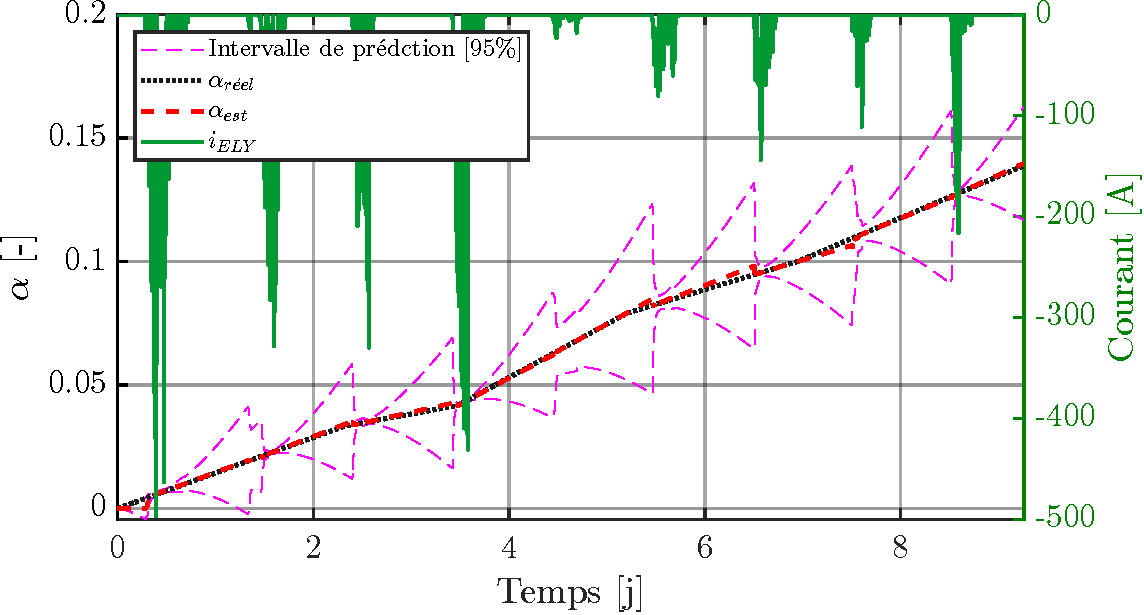
\includegraphics[width=\linewidth]{Chapitre 1/Diag_pac/Figures/comp_alpha_sigma_pemwe.pdf}
    \caption{Comparaison entre le paramètre de vieillissement réel $\alpha$ et son estimation par l'EKF pour le PEMWE.}
    \label{fig:ekf_ely}
\end{figure}
\FloatBarrier

% ------------------------------------------------------------
\subsection{Discussion}
% ------------------------------------------------------------

L'approche présentée dans cette section repose sur une hypothèse fondamentale~: le vieillissement des deux composants hydrogène peut être résumé par un unique paramètre scalaire $\alpha$, qui capture simultanément la dégradation de la résistance interne et du courant limite. Cette hypothèse de couplage linéaire entre les deux paramètres physiques est soutenue par plusieurs travaux expérimentaux~\cite{bressel_extended_2016}\cite{foniok_mechanisms_2025}, et présente l'avantage de réduire la dimension du problème d'estimation tout en conservant une interprétabilité physique directe.
Un aspect important de cette approche est la séparation des échelles de temps. Les résultats des observations de l'EKF ici peuvent localement perdre en précision lorsque les courants deviennent nuls et que le paramètre $\alpha$ devient inobservable, mais ces phases sont suffisamment peut espacées dans le temps pour considérer que le vieillissement (évoluant à des échelles de temps bien plus longues) peut être fidèlement suivi. Dans la suite de ce travail considérant des stratégies de gestion d'énergie, les décisions se prendront à l'échelle de l'heure et l'on considérera l'estimation des états de santé suffisamment fidèle pour pouvoir jouer un rôle dans la décision de contrôle. Il est également notable que les variations de $\alpha$ sont en réalité très lentes par rapport au pas de temps de contrôle, ce qui valide a posteriori l'hypothèse de quasi-stationnarité de $\beta$ et justifie la stabilité de l'algorithme d'estimation sur de longues durées.

% ------------------------------------------------------------
\subsection{Limitations}
% ------------------------------------------------------------

Plusieurs limitations de l'approche proposée méritent tout de même d'être soulignées. Premièrement, la réduction du vieillissement à un unique paramètre scalaire $\alpha$, bien que facilitatrice et bien fondée expérimentalement pour les piles à combustible~\cite{bressel_extended_2016}, constitue nécessairement une simplification. En réalité, les mécanismes de dégradation de la PEMFC et du PEMWE sont multiples et peuvent évoluer de manière indépendante selon les conditions d'utilisation~\cite{foniok_mechanisms_2025}\cite{endrodi_challenges_2025}. Des dégradations localisées, des empoisonnements de membrane ou des phénomènes de corrosion des électrodes, par exemple, ne sont pas capturés par ce formalisme scalaire. L'indicateur $\alpha$ doit donc être interprété comme un indicateur macroscopique de l'état de santé global du composant, et non comme une description fidèle de l'ensemble des mécanismes physiques sous-jacents.

Deuxièmement, l'observabilité de l'état $\alpha$ dépend de la richesse du signal d'excitation du composant. Comme mentionné ci-dessus, lors des phases où le courant est nul, l'influence de $\alpha$ disparaît du modèle de sortie, privant l'EKF de toute information utile. Dans un micro-réseau isolé à source solaire intermittente, ces phases d'inactivité peuvent être longues (nuits, périodes nuageuses prolongées). Un mécanisme d'inhibition ou de gel de la mise à jour de l'estimateur pendant ces phases permettrait d'éviter une dérive non physique de l'estimation.

Troisièmement, la méthode repose sur la précision du modèle paramétrique de tension~: toute erreur de modèle non capturable par $\alpha$ se traduit par un biais sur l'estimation. En particulier, l'hypothèse d'une évolution linéaire des paramètres avec le vieillissement peut être mise en défaut en fin de vie, où des phénomènes non linéaires et des dégradations irréversibles peuvent survenir~\cite{nguyen_comprehensive_2023}. Une extension vers des modèles de vieillissement non linéaires, ou vers des filtres de Kalman sans parfum (UKF, \textit{Unscented Kalman Filter})~\cite{chen_fuel_2019}, peut constituer une perspective pour améliorer la précision en fin de vie.

Enfin, les résultats présentés dans ce chapitre sont issus de simulations numériques utilisant des profils de consommation et d'irradiance représentatifs, mais non validés sur des données expérimentales réelles issues du micro-réseau de La Réunion. La validation expérimentale de l'algorithme d'estimation dans des conditions de fonctionnement réelles avec les bruits de mesure, les dérives instrumentales et la variabilité des profils d'utilisation qui leur sont propres constitue une prochaine étape avant un déploiement opérationnel.

\newpage